\chapter{Realidade aumentada}
\label{cap:realidadeaumentada}	
%	\epigraph{``Colocar algo aqui ''}{Autor}

	A Realidade Virtual utiliza a tecnologia com o propósito de simular uma inserção do usuário em um
	mundo virtual onde ele não conseguiria distinguir o cenário real daquele em que fora inserido, ou
	seja, o usuário estaria inserido em uma simulação de um mundo complemente sintético
	\cite{ronaldAzuma}. Esse mundo sintético pode imitar as propriedades de alguns ambientes
	encontrados no mundo real, podendo até exceder os limites da realidade física.
	
	Em contraste com a Realidade Virtual, a Realidade Aumentada permite ao usuário focar em seu
	ambiente físico e interagir em tempo real entre ambos os mundos. Essa nova forma de interação
	possibilita ao usuário manipular informações entre esses mundos de uma forma mais natural, ou seja,
	minimizando a necessidade de um treinamento para sua adaptação~\cite{kernerTori}. De forma geral,
	pode-se citar três características principais de aplicações desenvolvidas para a Realidade Aumentada:
	
	\begin{itemize}
	  \item Combinação entre o real e o virtual;
	  \item Interatividade em tempo real;
	  \item Possibilidade de visualização de objetos virtuais em 3D.
	\end{itemize}
	
	A Realidade Aumentada combina uma visão composta por cenas reais (visualizados pelo usuário) com
	objetos virtuais (gerados com auxílio do computador) para serem apresentadas ao usuário com o
	objetivo de inserir novas informações virtuais a respeito de objetos físicos visualizados por ele. O
	reconhecimento dos objetos físicos pode ocorrer através do uso marcadores, onde cada objeto físico possui
	seu marcador que o identifique e suas informações são apresentadas através de objetos virtuais.
	Tais informações são projetadas com o objetivo de melhorar a percepção sensorial do usuário com
	relação aos cenários obtidos pela integração do real com o virtual~\cite{tobias}.
	
	A Realidade Aumentada está inserida dentro de um conceito denominado Realidade Misturada. Esta
	é definida como um ambiente no qual os objetos pertencentes tanto mundo real quanto ao mundo
	virtual são apresentados de forma simultânea ao usuário. A Realidade Misturada visa complementar
	aspectos de ambos os mundos através do uso de informações incluídas em elementos virtuais. A
	figura~\ref{fig:diagramaRV} apresenta a divisão desses conceitos.
	
	\begin{figure}[htb]
		\centering 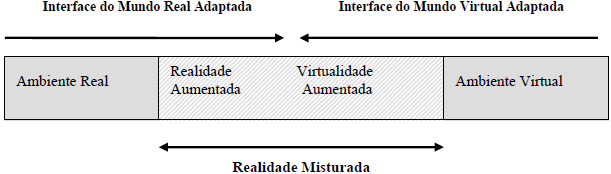
\includegraphics[scale=.8]{figuras/cap2/rv.jpg}
		\caption{\textit{Ambiente de Realidade Misturada ~\cite{kernerTori}}}
		\label{fig:diagramaRV} 
	\end{figure}
	
	\begin{enumerate}
	  \item \textbf{Ambiente Real:} Representa um ambiente constituído exclusivamente de objetos reais. 
	
	  \item \textbf{Realidade Aumentada:} Possui o ambiente real como interface de interação com o
	  usuário, com o propósito de inserir novas informações nele através de objetos virtuais.

	  \item \textbf{Virtualidade Aumentada:} A diferença entre a Realidade Aumentada e a Virtualidade
	  Aumentada está em sua forma de interação. Esta tem a finalidade de inserir elementos reais dentro
	  do mundo virtual e utilizar o ambiente virtual como interface de usuário. Para que isso ocorra, a
	  Virtualidade Aumentada utiliza técnicas computacionais para capturar elementos reais e inseri-los
	  no mundo virtual como objetos virtuais, como por exemplo, uma foto do usuário (objeto real) ser 
	  escaneada ou retirada através de uma~\textit{webcam} e ser inserida no mundo virtual para compor o
	  objeto virtual.

	  \item \textbf{Ambiente Virtual:} É definido como um ambiente compostos exclusivamente por objetos
	  virtuais, simulando um ambiente completamente sintético.
	
	\end{enumerate}
	
	Como um todo, os sistemas desenvolvidos para a Realidade Aumentada apresentam pontos chaves para
	seu funcionamento~\cite{henrysson}:
	
	\begin{enumerate}
	  \item \textbf{Rastreamento:} O sistema é responsável por obter as informações corretas a respeito
	  do posicionamento e orientação do usuário. A recuperação dessas informações torna-se necessária
	  		para a apresentação do conteúdo virtual correspondente. Nesta etapa são utilizados equipamentos
	  		(seção~\ref{sec:equipamentos}) responsáveis pela captura e processamentos dessas informações. O
	  		estabelecimento desses parâmetros é conhecido como \textit{tracking}. 
	  
	  \item \textbf{Registro:} Após o rastreamento ser concluído é feito o registro das informações
	  		correspondente a cada objeto reconhecido. O registro deve ser feito de modo que seja
	  		preservada a interatividade do usuário para que a relação entre o real e o virtual estejam
	  		alinhadas dentro de um mesmo domínio.
	  			
	  \item \textbf{Visualização:} A partir do resultado final gerado, esse sistema deve ser capaz de
	  produzir os objetos correspondentes em algum dispositivo que permita ao usuário visualizar tais
	  		informações.
	  
	\end{enumerate}
	
	O processamento destas imagens é constituído de etapas bem definidas
	(seção~\ref{sec:reconhecimentoMarcadores}), tendo como etapa inicial o reconhecimento dos
	marcadores utilizados pela Ralidade Aumentada e, posteriormente, a obtenção do código
	identificador do marcador. Por fim, a construção do objeto virtual correspondente.
	
	\section{Aplicações}
\label{sec:aplicacoes}

	Tendo em vista o potencial de aplicação da Realidade Aumentada na interação com usuários muitos estudos tem
	sido realizados neste sentido. Aplicações tem sido desenvolvidas em diversos ramos da atividade humana. 
	A seguir exemplifica-se alguns usos da Realidade Aumentada:
	
	\begin{itemize}
	  \item \textbf{Entretenimento} 
	  
	  		É nessa área que encontra-se o maior número de aplicações utilizando a Realidade
	  		Aumentada, sendo estas desenvolvidas principalmente para a área de jogos. O grande
	  		diferencial em utilizar a Realidade Aumentada em jogos é fazer com que seus cenários interajam
	  		com o mundo real ao qual o usuário está inserido. Isso possibilita uma interação maior
	  		do usuário e o cenário apresentado pelos jogos. 
	  		
	  \item \textbf{Medicina} 
	  
	  		O uso da Realidade Aumentada vem auxiliando a medicina em muitos aspectos, desde a visualização
	  		partes do corpo até a sua utilização em cirurgias. O \textit{HMD (Head Mounted Display)} é um
	  		equipamento bastante utilizado para auxiliar na visualização dos objetos virtuais,
	  		possibilitando que o mesmo seja seja utilizado em cirurgias guiadas por imagens. Deste modo,
	  		essa aplicação da Realidade Aumentada auxiliará em um melhor planejamento cirúrgico,
	  		contribuindo para uma diminuição dos riscos envolvidos~\cite{suthau, nilsson}.
	
	  \item \textbf{Mercado imobiliário e arquitetura} 
	  
	  		Maquetes e \textit{design} de interiores são construídas utilizando Realidade Aumentada com
	  		propósito de exemplificar aos consumidores o estado do empreendimento ao término de sua
	  		construção. Desta forma, a Realidade Aumentada é bastante utilizada nessas áreas para
	  		possibilitar aos compradores visualizar e customizar seus ambientes, possibilitando a
	  		modificação da disposição dos objetos e a observação dessas novas disposições.
	  		%com que o comprador faça modificações nas disposições dos objetos do jeito que achar
	  		% necessário e observar suas novas disposições.

	  \item \textbf{Auxílio na obtenção de informações a respeito de produtos} 
	  
	  		Empresas utilizam a Realidade Aumentada com o propósito de oferecer maiores detalhes a respeito
	  		de seus produtos. Eles são identificados por marcadores reconhecidos pela Realidade Aumentada.
	  		As informações necessárias são extraídas após o reconhecimento desse marcador e um objeto
	  		virtual contendo informações a respeito do produto é apresentado ao usuário. No caso de uma
	  		rede de supermercados, tais informações poderiam representar descontos, opiniões e ingredientes
	  		de produtos anunciados. Utilizando ainda o exemplo anterior, a localização dos produtos dentro
	  		do estabelecimento poderia ser mapeada de uma forma com que uma aplicação pudesse auxiliar o
	  		usuário a encontrar um determinado produto, através de uma navegação guiada por GPS
	  		ou por outros marcadores que guardariam a localização referentes a cada tipo de produto.
			
							  		
	  		%A visualização 3D do conteúdo interior de um produto a partir de marcadores posicionados nas
	  		%caixas do produto, proporcionou empresas utilizarem a realidade aumentada para possibilitar
	  		% com que os clientes possam obter maiores detalhes sobre o produto antes da compra.
	  
	  %%TODO arrumar a referência Augmented Reality Technology for Education, Mariano Alcatriz
	  % (procurar o bibtex)
	  \item \textbf{Educação}  
	  
	  		Através dos benefícios providos pela flexibilidade e usabilidade, a Realidade
	  		Aumentada foi utilizada na educação com o foco na aprendizagem. Sua utilização vai
	  		além da aprendizagem utilizando somente os livros, ela explora características que até então
	  		não eram percebidas no ambiente acadêmico, potencializando sua aprendizagem devido
	  		principalmente a interatividade provida pela Realidade Aumentada
	  		\cite{kaufmann,markBillinghurst}. Para exemplificar essa aplicação na Realidade Aumentada, 
	  		objetos dentro do museu britânico foram mapeados utilizando marcadores reconhecidos pela
	  		Realidade Aumentada proporcionando aos visitantes obterem informações a respeito dos objetos
	  		apresentados~\cite{museum}. Por outro lado, a Realidade Virtual vem sendo aplicada na educação
	  		desde a década de 90. Esses projetos proporcionam a criação de um mundo virtual com o propósito
	  		de ensinar e investigar os aspectos relacionados, como por exemplo, da cinemática,
	  		eletrostática, estruturas moleculares, estudo da biologia e matemática~\cite{ko, hannes}.
			
	  %% ~\cite{mariano}
	
	  \item \textbf{Turismo} 
	  
	  		Essa área tem sido bastante explorada devido a possibilidade de mapeamento de pontos
	  		turísticos e disponibilização de informações através desse mapeamento. Essas informações podem
	  		ser disponibilizadas de acordo com o perfil do usuário, com objetivo de auxiliá-lo na busca de
	  		locais de seu interesse. A localização desses pontos é feito através das coordenadas de
	  		localização do usuário, obtidas através de um GPS. Essas informações são cruzadas com posições
	  		de longitude, latitude e altitude obtidas de um banco de dados contendo todos os mapeamentos
	  		feitos. Na Realidade Aumentada essas posições mapeadas são denominadas de POI's (\textit{Points Of
	  		Interest}). Por causa da mobilidade obtida por esses recursos, eles são encontrados
	  		principalmente em aplicações voltadas para dispositivos móveis.
	
	\end{itemize}
	
	
	Como observado, a Realidade Aumentada é utilizada em diversas áreas com base em uma característica
	comum entre elas, a possibilidade de interação entre o real e o virtual. A visualização dos recursos
	providos pela Realidade Aumentada necessita de equipamentos compatíveis. Esses equipamentos
	proporcionam a captura de imagens, correspondente ao ambiente real do usuário, a construção e
	apresentação de objetos virtuais ao usuário.
	

	\section{Equipamentos}
\label{sec:equipamentos}

	Como etapa inicial para o funcionamento da Realidade Aumentada, necessita-se de equipamentos que
	possuam a funcionalidade de captura de vídeo, como por exemplo~\textit{webcam's}. Esses
	proporcionam a captura do ambiente do usuário e envia os dados para um dispositivo responsável pelo
	processamento. Dentre os equipamentos utilizados inicialmente na Realidade Aumentada pode-se citar
	o~\textit{HMD (Head Mounted Display)}. Eles eram utilizados com o objetivo de captura das
	informações, através de suas câmeras acopladas, posteriormente processavam as informações
	necessárias e exibia o resultado do processamento ao usuário através de objetos virtuais
	visualizados em suas telas acopladas ao equipamento.
	
	Este equipamento é fixado na cabeça do usuário podendo ter o formato de um capacete ou de um
	óculos. Algumas utilidades desse equipamento pode ser encontrada em realizações de simulações
	computadorizadas e também para a visualização dos objetos virtuais ao qual o âmbito da Realidade
	Aumentada está inserida~\cite{ronaldAzuma}.
		
	Quando esse equipamento foi proposto, ele possuía algumas desvantagens por ser muito pesado e
	evasivo. Atualmente, projetos estão sendo desenvolvidos para tentar minimizar essas desvantagens. A
	figura~\ref{fig:hmd} mostra um equipamento~\textit{HMD} com características que favoreçam sua
	utilização. Por outro lado, a grande vantagem desse tipo de equipamento é a possibilidade de
	imersão do usuário em um ambiente onde ele consiga interagir entre o virtual e o real de uma forma
	mais natural.
	
	\begin{figure}[htb]
		\centering 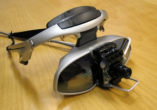
\includegraphics[scale=1.25]{figuras/cap2/hmd.jpg}
		\caption{\textit{Head Mounted Display ~\cite{nilsson}.}}
		\label{fig:hmd} 
	\end{figure}
	
	Atualmente, os \textit{smartphones} estão ganhando cada vez mais espaço dentro da Realidade
	Aumentada. Com a evolução do \textit{GPU (Graphics Processing Unit)} nestes, ocorreu a
	popularização de seu uso em aplicações voltadas para a Realidade Aumentada. A grande vantagem em
	sua utilização está na abrangência com que eles são distribuídos e principalmente na mobilidade
	conseguida através dos mesmos. Este equipamento comporta todos os recursos necessários para sua
	utilização na Realidade Aumentada:
	
	\begin{enumerate}
	  	\item A câmera do celular substitui a \textit{webcam} ou as câmeras acopladas ao HMD;
		\item O processamento gráfico é feito na~\textit{GPU};
		\item O resultado é apresentado no próprio visor do aparelho, suprindo a necessidade de um
		monitor ou telas para a visualização do objeto virtual.
	\end{enumerate}

	Um exemplo de utilização da Realidade Aumentada em \textit{smartphones} pode ser visto na
	figura~\ref{fig:arAndroid}. Nesta, a câmera do \textit{smartphone} captura a imagem do marcador,
	processa as informações necessárias e exibe um carro como objeto virtual correspondente para aquele
	marcador.
						
	\begin{figure}[htb]
		\centering 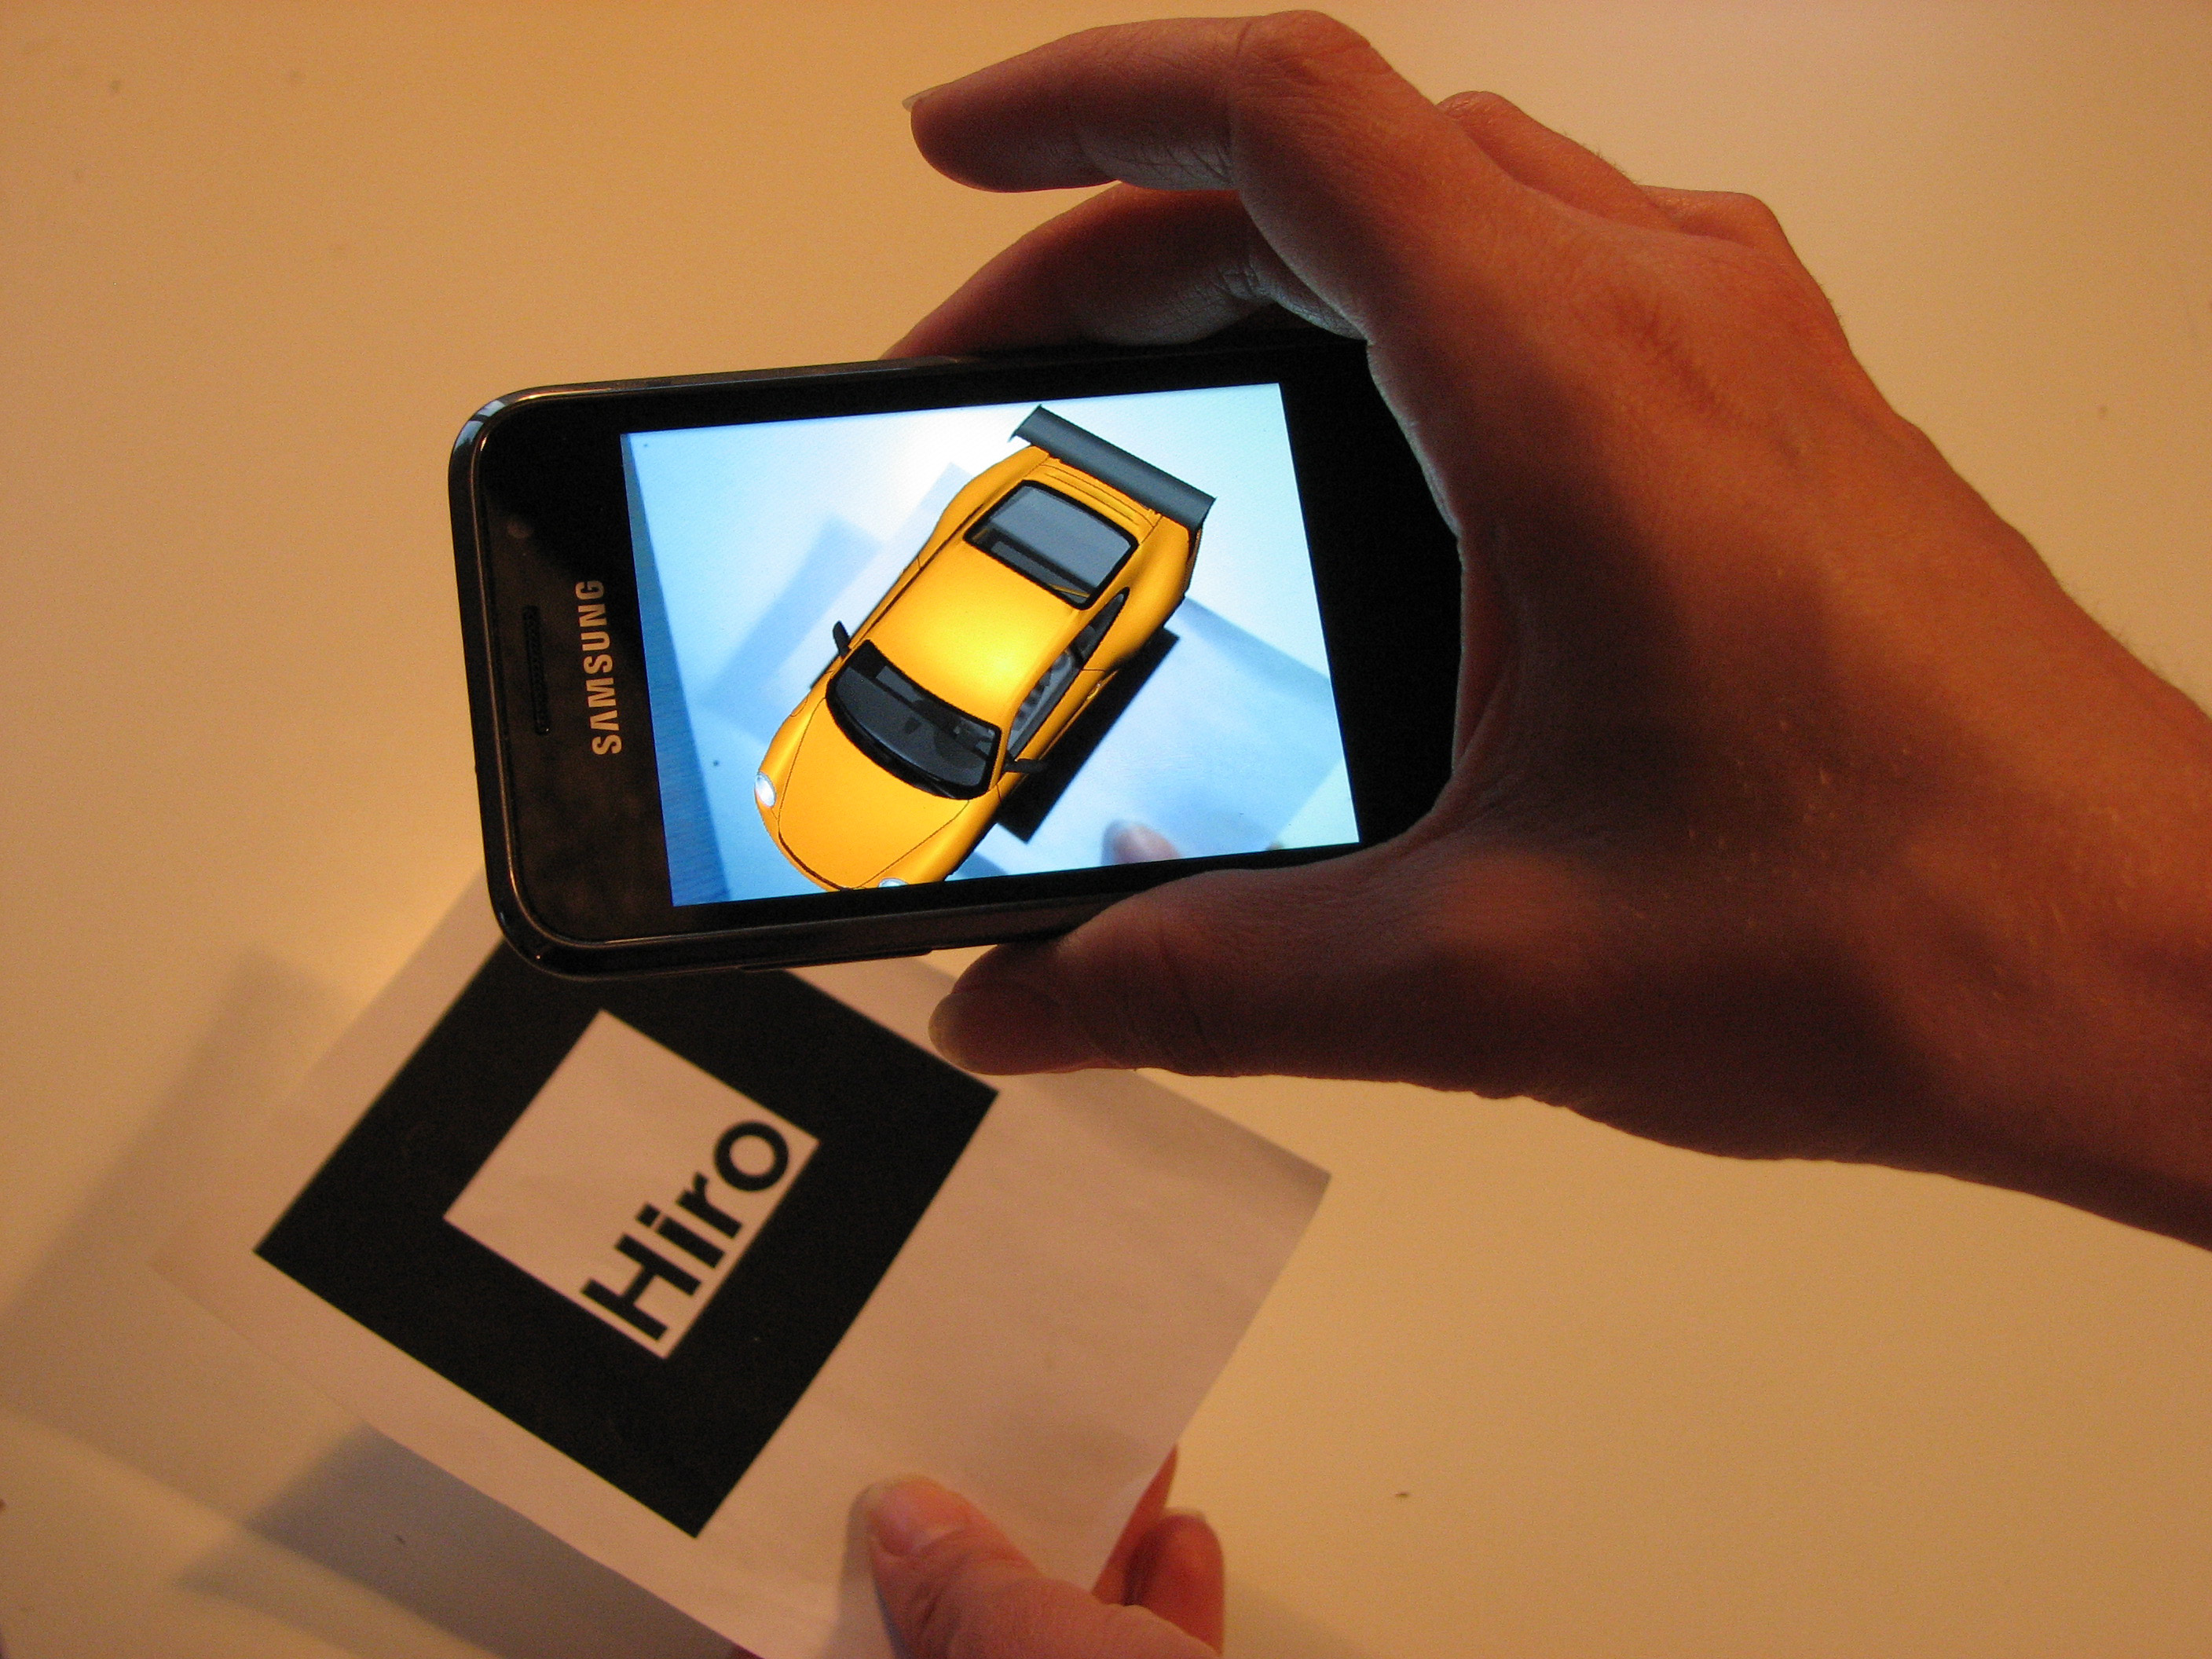
\includegraphics[scale=0.1]{figuras/cap2/ARToolKit-car-Android.jpg}
		\caption{\textit{Exemplo de utilização de smartphone na Realidade Aumentada~\cite{arToolWorks}.}}
		\label{fig:arAndroid}
	\end{figure}
	\section{Classificação}
\label{sec:classificacao}
	
	Com a evolução dos equipamentos, a visualização dos objetos virtuais torna-se cada vez mais real.
	Através desses equipamentos, os sistemas de Realidade Aumentada podem ser classificados de acordo
	com a forma como que o usuário vê o mundo misturado. Em~\cite{ronaldAzuma} é apresentado uma
	divisão para classificações entre as tecnologias óptica e vídeo. Essas classificações variam de
	acordo com o tipo de equipamento utilizado e com o tipo de sistema de visualização:
	
	\begin{enumerate}
		\item \textbf{Visão direta}
		
		Também conhecida como visão imersiva, nesta classificação os objetos virtuais são visualizados
		na mesma direção com que as cenas reais são capturadas. Esta classificação é utilizada
		principalmente em equipamentos que capturam as imagens reais, processam as informações
		necessárias e apresentam objetos ao usuário no mesmo equipamento~\cite{suthau}. Por
		exemplo, a utilização de equipamentos do tipo \textit{HMD} proporciona ao usuário uma visão
		direta, tendo em vista que a captura das cenas e a apresentação do objeto virtual foi feito pelo
		mesmo equipamento. Desta forma o usuário não necessita desviar o foco do mundo real a fim de
		observar as informações providas pelo objeto virtual.
		
		%Isso proporciona com que o usuário não precise desviar o olhar para a visualização do objeto
		% virtual.
		
		\item \textbf{Visão indireta}
		
		Ocorre quando a visualização do mundo misturado é feita através de algum dispositivo e a
		apresentação dos objetos virtuais, correspondentes as cenas, seja feita em um outro dispositivo,
		ocasionando o desvio da atenção do usuário~\cite{suthau, kernerTori}. Um exemplo para
		esse tipo de classificação é observado quando a captura das imagens reais é feita através de uma
		\textit{webcam}, processadas em um computador e o resultado apresentado em projeções ou em
		monitores.
		
	\end{enumerate}
	
	Uma outra forma de se classificar a Realidade Aumentada baseia-se nos sistemas utilizados por ela.
	Estes podem ser classificados de acordo com o tipo de equipamento utilizado para captura de cenas
	reais, processamento e os equipamentos responsáveis pela visualização do objeto virtual. Estas
	classificações abrangem tanto sistemas que utilizem visão óptica quanto visão por vídeo. Sendo
	classificados em:
		
	\begin{enumerate}
	
		\item \textbf{Visão direta por vídeo} 
		
		Neste tipo de classificação, equipamentos \textit{HMD} são utilizados para o recebimento direto
		da imagem real através de suas câmeras acopladas. As imagens capturadas são processadas em
		um gerador de cenas e as informações virtuais geradas por este são apresentadas diretamente ao
		usuário, através das telas acopladas ao equipamento. 
		
		%Nesta, um equipamento é utilizado para combinar cenas reais com as virtuais, a partir de
		%imagens obtidas através desse equipamento composto por pequenas câmeras de vídeo. As imagens
		%capturadas são processadas e novas informações virtuais são geradas por um computador. Essas
		%informações são misturadas com as cenas reais capturadas pelas micro câmeras acopladas ao
		%equipamento e as novas informações geradas pelo gerador de cenas são mostradas diretamente ao
		%usuário através das telas acopladas ao equipamento.
		
		\item \textbf{Visão direta por óptica} 
		
		De forma análoga a visão direta por vídeo, esta possui as mesmas etapas para obtenção e geração
		as informações virtuais a serem apresentadas ao usuário. No entanto, as informações geradas são
		apresentadas ao usuário através de lentes ou espelhos. Estas são inclinadas e posicionadas
		para que a projeção das imagens vindas do monitor acoplado seja refletida e redirecionada para
		os olhos do usuário.
		
		\item \textbf{Visão por vídeo baseada em monitor} 
		
		Após a captura das cenas, os objetos virtuais são gerados no gerador de cenas e misturados com
		as cenas reais no combinador de cenas. As informações geradas são apresentadas ao usuário
		através de um monitor.
		
		\item \textbf{Visão por óptica baseada em projeção} 
		
		Nessa classificação, as imagens dos objetos virtuais são apresentadas sem a necessidade de um
		equipamento específico. As mesmas são processadas em computador e projetadas em superfícies do
		ambiente real, por causa da necessidade de superfícies específicas para projeções, essa
		classificação torna-se mais restrita em comparação com as demais classificações.
		
	\end{enumerate}

	\section{Marcadores}
\label{sec:marcadores}

	Atualmente, é possível encontrar aplicações que utilizam padrões de símbolos bidimensionais para
	compor informações e transportar as mesmas de uma forma mais simplificada, a exemplo dos
	padrões~\textit{QRCode, PDF147} e~\textit{DataMatrix}~\cite{gao}. Alguns padrões permitem que as
	informações estejam representadas de forma redundante, pois auxiliam em sua detecção e na correção
	de possíveis erros. No âmbito industrial, seu campo de aplicação varia de acordo com a necessidade
	de cada sistema, como por exemplo transportar informações em etiquetas. Outros tipos de marcadores
	são utilizados para representar dados de localização e reconhecimento de objetos, como visto na
	Realidade Aumentada.
	
\subsection{Símbolos bidimensionais}
	\label{sec:simbolos_bidimensionais}
	
	Esse tipo de código de barras foi desenvolvido por volta de 1987. No código de barras bidimensional
	as informações são armazenadas tanto na altura quanto na largura, por essa razão possui uma maior
	capacidade de armazenamento das informações quando comparada aos símbolos unidimensionais. Os
	modelos de códigos unidimensionais armazenam as informações em apenas em uma dimensão, por
	causa dessa característica há uma limitação na quantidade de informação ser armazenada
	por eles, de acordo com cada padrão.  
	
	Para exemplificar essas características é apresentada a figura~\ref{fig:simbolos} ilustrando
	esses dois tipos de símbolos. O código apresentado na figura~\ref{fig:barcode} corresponde a um
	símbolo unidimensional, a altura desse símbolo (representado no eixo vertical) fornece
	redundância e legibilidade, possibilitando um tempo de resposta rápida, uma vez que a análise é
	feita em uma dimensão. Devido a limitação no armazenamento das informações por ele, geralmente são
	guardados valores chaves que possibilitem a busca de informações correspondentes ao código em um
	banco de dados específico. A figura~\ref{fig:datamatrix} apresenta um símbolo bidimensional
	denominado~\textit{DataMatrix}, as informações contidas neste são armazenadas em ambos os eixos
	horizontal e vertical, otimizando o espaço utilizado por ele, possibilitando a inserção de
	caracteres alfanuméricos, bem como um mecanismo responsável pela correção das informações obtidas
	através do processo de decodificação. Em contraste com esse modelo encontrado nos códigos
	unidimensionais, as informações armazenadas por esse símbolo remete a um conceito de banco de dados
	portátil e não somente o conceito de chave como apresentado no modelo unidimensional, podendo 
	armazenar uma maior quantidade de informação~\cite{gao}.
	
	\begin{figure}[htb]
		\centering
			\subfloat[\textit{BarCode} \cite{ean13}]{
				\label{fig:barcode}
				\centering 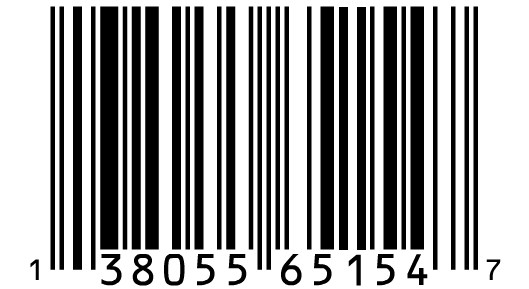
\includegraphics[scale=0.3]{figuras/cap2/codigo_barras.jpg}
			}
			\subfloat[\textit{DataMatrix} \cite{gao}]{
				\label{fig:datamatrix}
				\centering 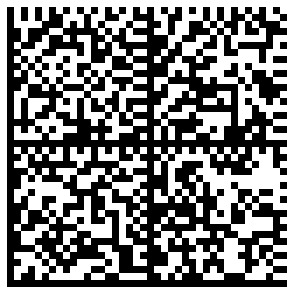
\includegraphics[scale=0.4]{figuras/cap2/datamatrix.jpg}
			}
		\caption{\textit{Exemplos de símbolos unidimensional e bidimensional.}}
		\label{fig:simbolos} 
	\end{figure}
	
	Os códigos bidimensionais podem ser divididos em duas categorias. A primeira denominada
	~\textit{stacked code} e a segunda chamada de~\textit{matrix code}. A diferença entre essas
	categorias está na sua composição. Enquanto que a~\textit{stacked code} trabalha com simbologias
	compostas por uma série de código de barras unidimensionais empilhadas uma em cima das outras,
	a~\textit{matrix code} codifica os dados com base nas posições dos pontos negros definidos dentro
	de uma matriz. Isso faz com que cada elemento da matriz possua a mesma dimensão, desta forma a
	decodificação é calculada em relação a posição do elemento preenchido na matriz. A
	tabela~\ref{tab:exemplo} apresenta alguns tipos de códigos bidimensionais e a categoria
	correspondente a cada código listado.
	
	
	\begin{table} % aqui começa o ambiente tabela
		\centering
		\caption{Códigos bidimensionais e suas categorias.}
		\begin{tabular}{lcc} 
			\hline % este comando coloca uma linha na tabela
			\textbf{Código bidimensional} & \textbf{Categoria} \\ 
			%\textit{\textbf{Stacked code}} & \textit{\textbf{Matrix code}}	\\
			\hline
			\hline
			\textit{Code 49} & \textit{Stacked} \\
			\textit{Data Matrix} & \textit{\textit{Matrix}} \\
			\textit{Portable Data File 417 (PDF417)} & \textit{Stacked}  \\
			\textit{QRCode} & \textit{\textit{Matrix}}\\
			\hline
		\end{tabular}
		\label{tab:exemplo}
	\end{table}
	
	A figura \ref{fig:qrCode} exemplifica um código de barras bidimensional da 
	categoria~\textit{matrix code}. Esse tipo de código é denominado de \textit{QRCode (Quick Response Code)}. 
	O \textit{QRCode} foi desenvolvido no Japão, no ano de 1994 com o objetivo de ser um código que possibilitasse um
	bom armazenamento de informações, compacto e que oferecesse uma leitura rápida e de fácil acesso.
	Este código pode codificar até 7089 caracteres numéricos (somente números), 4296 caracteres alfanuméricos 
	(letras e caracteres ASCII) ou 2953 \textit{bytes} de dados binários (\textit{bytes} hexadecimal)~\cite{kato}. Possui um 
	formato quadrático com dimensões variando
	de 21 x 21 até 177 x 177 células (conforme a versão do~\textit{QRCode}), onde cada célula codifica
	um \textit{bit}. É oferecido quatro níveis de detecção e correção de erros, possibilitando a
	recuperação de informações de regiões danificadas do código. A tabela~\ref{tab:nivelFalha}
	exemplifica esses níveis e apresenta a porcentagem de recuperação das informações oferecida por
	cada nível.
	
	
	\begin{table}
		\centering
		\caption{Níveis de correção de erros suportado pelo QRCode~\cite{kato}.}
		\begin{tabular}{lcc} 
			\hline
			 \textbf{Nível} & \textbf{Porcentagem de informação recuperada} \\
			\hline
			\hline
			\textit{Low} & 7\% \\
			\textit{Medium} & 15\% \\
			\textit{Quality} & 25\% \\
			\textit{High} & 30\% \\
			\hline
		\end{tabular}
		\label{tab:nivelFalha}
	\end{table}
	
	
	O \textit{QRCode} possui características estruturais com o objetivo de facilitar sua identificação
	e obtenção das informações necessárias para a sua correta decodificação. Tais características
	estão ilustradas na figura~\ref{fig:qrCode}.
				
	\begin{figure}[htb]
		\centering 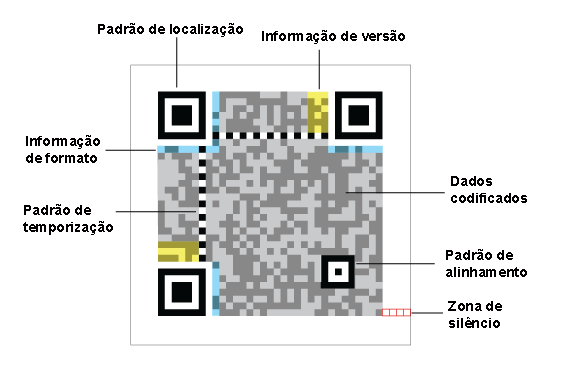
\includegraphics[scale=0.6]{figuras/cap2/qranatomy.png}
		\caption{\textit{Ilustração das propriedades estruturais do QRCode. Adaptado de~\cite{qrcodespec}.}}
		\label{fig:qrCode} 
	\end{figure} 
	
	\begin{itemize}
	  \item \textit{Padrão de localização}
			  
	  	Esse padrão baseia-se nas posições dos três vértices localizadas nos cantos do símbolo. A
	  	partir desses três pontos é possível estimar o quarto canto da imagem, por consequência a
	  	posição, tamanho e o centro dos símbolos podem ser detectados, sendo assim utilizado para
	  	referência posicional do símbolo. Desta forma, o reconhecimento pode ser feito em todas as
	  	direções.
				  
		\item \textit{Padrão de temporização}
				  
		Padrão responsável pela identificação e correção das coordenadas centrais de cada célula. Este
		padrão é utilizado quando o símbolo está distorcido, possibilitando a identificação do espaçamento
		entre as células.
					
		\item \textit{Padrão de alinhamento}
					
		Por fim, a correção de distorção, especialmente a não linear, é feita através desse padrão. 
		Essa visa corrigir a distorção do símbolo quando este estiver em uma superfície curva ou 
		com o leitor inclinado.	Por fim, esta célula facilita a obtenção da coordenada central do padrão 
		de alinhamento.
		
		\item \textit{Dados codificados}
		
		É a região responsável pelo armazenamento dos dados codificados.
		
		\item \textit{Informação de formato}
		
		Contém a taxa de correção de erro e o padrão de máscara utilizado.
		
		\item \textit{Zona de silêncio}
		
		É a margem ao redor do \textit{QRCode} necessário para que o código seja lido corretamente. Possui
		a medida correspondente a quatro células de largura.
		
		\item \textit{Informação de versão}
		
		Responsável pela identificação da versão utilizada pelo \textit{QRCode}, podendo variar a partir
		da versão 1 (correspondente a 21 x 21 células) até a versão 40 (correspondente a 177 x 177
		células). As versões possuem a mesma estrutura, porém a capacidade de armazenamento varia de uma
		versão para outra.
									
	\end{itemize}
	
	A tabela \ref{tab:tabelaCodigos} mostra um comparativo entre diferentes tipos de códigos tanto
	unidimensionais (\textit{barcode}) quanto bidimensionais (\textit{QRCode} e \textit{Data Matrix}).
	As quantidade de referência internas apresentadas na tabela dizem respeito a pontos contidos
	internamente dentro do código cujo propósito seja o auxílio para obtenção do correto
 	posicionamento do mesmo. Também é mostrada a diferença na quantidade de informação armazenada por
	esses códigos.
	
	
	\begin{table} % aqui começa o ambiente tabela
		\centering
		\caption{Comparação de vários códigos \cite{marlon}.}
		\begin{tabular}{lccc} 
			\hline % este comando coloca uma linha na tabela
			 & \textbf{\textit{Barcode}} & \textbf{QRCode} & \textbf{\textit{DataMatrix}} \\
			\hline
			\hline
			Capacidade de armazenamento & 1\textit{byte}/4cm	 & 2953 \textit{bytes} & 2335 \textit{bytes} \\
			Velocidade de leitura & Rápido & Rápido & Lenta\\
			Especificação aberta & Sim & Sim & Sim\\
			Referências internas & 0 & 3 & 2 \\ 
			Recuperação dos dados & Não & Até 30 \%  & Até 30 \% \\
			Formato & Linear & Quadrado & Retangular\\
			\hline
		\end{tabular}
		 % igual ao ambiente figura
		\label{tab:tabelaCodigos}
	\end{table}
	
\subsection{Marcadores para Realidade Aumentada}
\label{sec:marcadoresRA}
		
		Cada aplicação voltada para a criação e/ou detecção de marcadores pode possuir seus próprios
		padrões de marcadores e algoritmos para seu reconhecimento. A área de definição de marcadores
		utilizados ainda está em aberto, com espaço para melhorias de acordo com cada aplicação~\cite{fpga}. Dentro
		desse universo pode-se citar as aplicações ARToolkit~\cite{artoolkit}, ARTag~\cite{artag} e
		ARToolkitPlus~\cite{kler}.
		
		De uma forma geral, para os objetos sejam reconhecidos como potenciais marcadores por
		essas aplicações, estes necessitam de um formato padrão constituído por uma ``moldura''
		confeccionada com bordas quadradas, de preferência na cor preta, pois algumas aplicações convertem
		as cores da imagem em uma escala de cinza. A construção e decodificação do conteúdo interior do
		marcador pode variar de acordo com cada aplicação, possibilitando uma flexibilização na construção
		do mesmo. Na abordagem da aplicação ARToolkit, o centro desses marcadores pode ser constituído por
		uma figura. Já no ARToolkitPlus, o interior dos marcadores é preenchido por quadrados de cor
		preta, podendo formar figuras geométricas diversas. Exemplos de marcadores utilizados por essas
		aplicações são apresentados na figura~\ref{fig:marcadoresAR}. 
		
		\begin{figure}[htb]
			\centering
				\subfloat[ARToolKit \cite{artoolkit}]{
					\label{fig:artoolkit}
					\centering 
\includegraphics[scale=1]{figuras/cap2/arToolkitMarker.png}
				}
				\subfloat[ARTag \cite{artag}]{
					\label{fig:artag}
					\centering 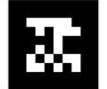
\includegraphics[scale=1]{figuras/cap2/arTagMarker.png}
				}
				\subfloat[ARToolkitPlus \cite{kler}]{
					\label{fig:artoolkitplus}
					\centering 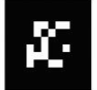
\includegraphics[scale=1]{figuras/cap2/arToolkitPlusMarker.png}
				}
			\caption{\textit{Exemplo de alguns marcadores utilizados na realidade aumentada.}}
			\label{fig:marcadoresAR} 
		\end{figure}
		
	Fazendo uma comparação entre esses marcadores e o \textit{QRCode} é possível observar que, da mesma
	forma como acontece com o código unidimensional apresentado na tabela~\ref{tab:tabelaCodigos},
	estes não possibilitam a recuperação de informações danificadas, mas possibilitam a identificação do erro. 
	Desta forma o não reconhecimento de parte do marcador pode comprometer todo o processo de reconhecimento. 
	Diferentemente do \textit{QRCode}, esses marcadores possuem uma capacidade bastante limitada para 
	armazenamento de informações. Por causa dessa limitação a maioria dos marcadores guardam somente um código
	identificador. Entretanto, são menos sensíveis a distorções de ângulo devido sua simplicidade. 
	

	\section{Reconhecimento de marcadores}
\label{sec:reconhecimentoMarcadores}	
	
		O processo de reconhecimento dos marcadores é dividido em etapas bem definidas. No entanto, estas
		podem ser implementadas de formas diferentes levando-se em consideração a aplicação utilizada.
		Esse processo tem o objetivo de identificar objetos com formatos pré-definidos e que possuam
		códigos de identificação compatíveis com a aplicação. A partir desse
		reconhecimento é possível estabelecer o posicionamento dos objetos em relação ao dispositivo
		responsável pela captura da imagens e apresentar o objeto virtual correspondente sobreposto ao
		marcador reconhecido. As etapas envolvidas nesse processo são apresentadas na
		figura~\ref{fig:pipelineAR} e dividas da seguinte maneira:
		
		\begin{figure}[htb]
			\centering 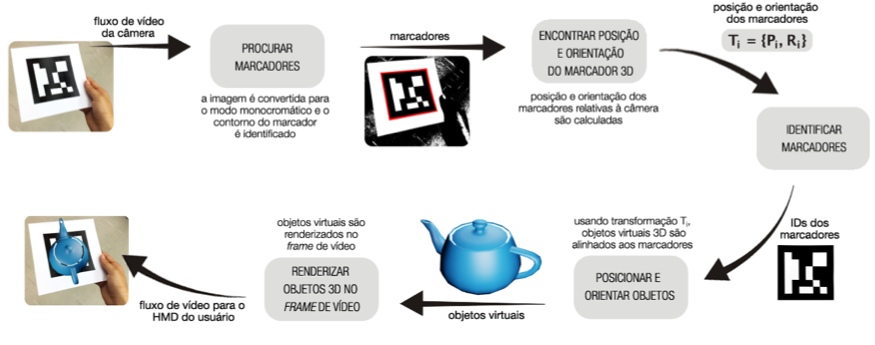
\includegraphics[scale=.55]{figuras/cap2/pipelineAR.png}
			\caption{\textit{Etapas do processo de reconhecimento de marcadores na Realidade
			Aumentada~\cite{fpga}.}}
			\label{fig:pipelineAR} 
		\end{figure}
		
		\begin{enumerate}
		  \item \textbf{Procurar marcadores}
		  
				O fluxo de vídeo obtido por uma câmera é entrada da etapa inicial do processo de
				reconhecimento. Ele é lido e encaminhado para o sistema de rastreamento. Neste, aplica-se uma
				operação de detecção de bordas como uma etapa inicial. Faz-se um reconhecimento de
				cada~\textit{pixel} dentro de um segmento para que seja feita um agrupamento de~\textit{pixels},
				a fim de se achar uma forma quadrangular e reconhecer a figura como um possível marcador. Esse
				método acaba sendo mais eficaz quando comparado com o método de derivar o marcador a partir de
				uma intensidade de luminosidade de escala de cinza, devido o seu reconhecimento em ambientes de
				pouca luminosidade e problemas relacionados com oclusão (parte da visualização do marcador é
				obstruída por um outro objeto)~\cite{artag}.
				
			\item \textbf{Encontrar posição e orientação do marcador 3D}
			
				Nesta etapa o marcador já foi encontrado na imagem. Para obter uma estimativa da posição do
				marcador é necessário obter quatro pontos não lineares e identificáveis na imagem. Estes pontos
				devem aproximar a um formato correspondente a um quadrado. Na situação de identificação das
				posições baseados na utilização de várias câmeras, envolve a localização do mesmo recurso em
				duas imagens obtidas por câmeras diferentes. Isso possibilitaria estimar a posição geométrica
				tridimensional de um recurso. Neste caso para estimar a localização de tal recurso necessitaria
				combinar as informações de três pontos não lineares. Alguns problemas podem ser detectados, como
				por exemplo, a distorção de perspectiva ocorrendo quando o plano da tela não é o mesmo plano do
				marcador~\cite{kler}.
				
			\item \textbf{Identificar marcadores}
			
				É nesta etapa que acontecem mais particularidades para o reconhecimento dos marcadores
				observadas em diferentes aplicações. Na aplicação ARTag, o conteúdo extraído do interior do
				marcador é preenchido com uma matriz quadrada 6 x 6 com células de cores preto e branco, aos
				quais representarão valores binários de 0's e 1's. Essa matriz retornará uma sequência de
				36~\textit{bits}, sendo analisada de quatro formas distintas por causa das quatro rotações
				possíveis para o marcador.
				
				O código identificador do marcador é constituído por 10 \textit{bits}, sendo codificado a
				partir da sequência dos 36~\textit{bits} obtidos e deixando os 26~\textit{bits} restantes para a
				detecção e correção de erros, bem como a unicidade em torno das quatro possibilidades de rotação
				do marcador~\cite{hirzer}. São utilizados os métodos~\textit{CRC (Cyclical Redundancy Check)}
				e~\textit{Forward Error Correction} para detecção do marcador e extração do seu número
				identificador correspondente, adicionando o conceito dos operadores lógicos XOR para codificação
				e decodificação. A correção e reparo dos erros, desalinhamento de fronteira, oclusão, dentro
				outros, fica sobre a responsabilidade do~\textit{FEC (Forward Error Correction)}. Outros
				métodos, baseados em probabilidades, também são aplicados para garantir o reconhecimento correto
				do identificador do marcador em relação aos demais marcadores.
				
				A figura \ref{fig:artagDecoding} exemplifica os passos necessários utilizado pelo ARTag para
				obter o código de identificação do marcador a partir do marcador reconhecido nas etapas anteriores 
				do~\textit{pipeline}.
				
				\begin{figure}[h]
					\centering 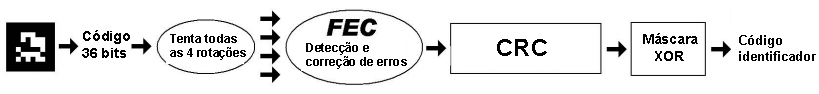
\includegraphics[scale=.55]{figuras/cap2/artag_decoding.png}
					\caption{\textit{Obtenção do código identificador do marcador. Adaptado de~\cite{artag}.}}
					\label{fig:artagDecoding} 
				\end{figure}
				
				De forma análoga, o ARToolkit extrai o conteúdo do interior do marcador e gera uma matriz
				quadrada. No entanto, as dimensões dessa matriz são de 16 x 16 ou 32 x 32. Os valores obtidos
				por essa matriz geram um vetor característico que é comparado com uma biblioteca de vetores
				característicos conhecidos e geram como resultado um fator de confiança para dizer se o
				marcador foi reconhecido.
				
			\item \textbf{Posicionar e orientar objetos}
			
				Nesta etapa, os objetos virtuais 3D são identificados e associados de acordo com o marcador
				identificado na etapa anterior. Os mesmos são alinhados ao marcador pelo posicionamento obtido na
				etapa 2.
			
			\item \textbf{Renderizar objetos 3D no ~\textit{frame} de vídeo}
			
				Por fim é gerado o \textit{frame} de vídeo, contendo o marcador e seu respectivo objeto virtual
				3D. Após ser renderizado, o mesmo é repassado para o objeto de visualização de vídeo, podendo ser um
				monitor,~\textit{HMD} ou \textit{smartphone}.
				
		\end{enumerate}
	
		A quantidade de marcadores, aos quais podem ser geradas com uma boa qualidade de reconhecimento
		varia para cada tipo de aplicação. Essa qualidade de reconhecimento refere-se a símbolos no
		interior dos marcadores aos quais são facilmente distinguíveis pelas aplicações. Isso mostra 
		que a quantidade de \textit{bits} obtidos a partir da matriz gerada pelo interior do marcador,
		pode-se construir diversos símbolos. No entanto, pela isomorfia dos marcadores (rotação do marcador 
		em 0, 90, 180 e 270 graus) muitos símbolos acabam sendo descartados por se tratar do mesmo marcador. 
		No ARTag e no ARToolkitPlus, esses números são bastantes diferentes.
		Enquanto que no primeiro, 2002 marcadores são reconhecidos facilmente, no segundo esse número cai
		para 512. Porem, muitos outros símbolos podem ser gerados, mas sem muita garantia de uma boa
		qualidade em seu reconhecimento. Não foi possível obter as mesmas informações a respeito da
		quantidade de marcadores que são reconhecidos pelo ARToolkit.
		
	
	
	\section{Trabalhos correlatos}
\label{sec:trabalhosRelacionados}

	O aumento da mobilidade no ambiente de trabalho de usuário, proporciona uma	abstração de diferentes 
	configurações de um ambiente, sendo suportado pelas diversas tecnologias de comunicação sem fio utilizadas na
	computação móvel. Desta maneira, vários trabalhos estão sendo desenvolvidos utilizando esta
	computação com o propósito de auxiliar o usuário na solução de seus problemas. Serão apresentados
	trabalhos que utilizam a computação móvel, aplicadas a ambientes ubíquo.
	 
	\subsection{\textit{CyberCode}}
\label{sec:cybercode}
	
	Em \cite{rekimoto} é apresentado uma proposta de utilização de marcadores baseados em códigos
	bidimensionais, denominado de CyberCode. Nesta aplicação as informações são codificadas em um
	padrão bidimensional para ser reconhecido por dispositivos de baixo desempenho. As informações
	correspondente aos marcadores são armazenados em um banco de dados, possibilitando assim a
	alteração dos dados de forma dinâmica, sem a necessidade de alterar o marcador. A
	figura~\ref{fig:cybercode} mostra um exemplo do marcador CyberCode.
	
	\begin{figure}[htb]
		\centering 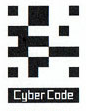
\includegraphics[scale=1]{figuras/cap2/cybercode.png}
		\caption{\textit{Exemplo de um marcador CyberCode \cite{rekimoto}.}}
		\label{fig:cybercode} 
	\end{figure} 
	 
	O uso dos mesmos pode ser combinado com outras tecnologias de rastreamento, com o objetivo de
	auxiliar o usuário na navegação em um ambiente específico. Desta maneira, eles seriam
	reconhecidos com o propósito de obtenção da localização do usuário no espaço. Com isso seria
	possível apresentar as informações ao usuário a respeito dos demais locais próximos a ele.
	
	Uma outra proposta para esses marcadores diz respeito a utilização dos mesmos para o mapeamento dos
	dispositivos. A própria equipe construiu um dispositivo de fácil manuseio constituído por uma
	câmera e um visor, denominado de \textit{InfoPoint}. Esse dispositivo capta a imagem correspondente
	ao marcador, acessa um banco de dados para extrair o conteúdo correspondente e apresenta o conteúdo
	correspondente no visor do dispositivo. Através desse dispositivo, o usuário é capaz de selecionar
	um marcador específico e transferir dinamicamente o conteúdo relativo a esse CyberCode para um outro
	marcador.
	
	\subsubsection{Aplicado à computação ubíqua}
	 
	A integração desse projeto com a computação ubíqua ocorre através da utilização de uma mesa
	digital. Sobre esta são acopladas câmeras com o propósito de reconhecer os objetos
	distribuídos em sua superfície. Após o reconhecimento de um novo dispositivo marcado por um
	CyberCode são apresentadas as informações correspondente ao objeto reconhecido. 
	
	Também é apresentada a utilização da mesa através da integração com um \textit{notebook}. O
	\textit{notebook} é reconhecido através do seu marcador associado, posteriormente é feita uma busca
	das informações relativas ao dispositivo, como por exemplo seu endereço~\textit{IP} e o
	posicionamento relativo a mesa digital. Desta forma, o \textit{notebook} estará integrado com a
	rede local juntamente com os objetos físicos reconhecidos pela mesa.
	
	Essa integração possibilita uma troca de informações livre entre os dispositivos. No exemplo
	anterior, o recurso de tela do \textit{notebook} foi estendido para a mesa digital. Isso
	possibilita com que o usuário utilize os recursos da mesa digital para interagir com o
	\textit{notebook}. Por exemplo, caso o usuário sinta a necessidade de mover o cursor do
	\textit{notebook}, ele poderá utilizar a sensibilidade da mesa para mover o cursor dentro do espaço
	delimitado como extensão da tela do \textit{notebook}.
	

	\subsection{\textit{HELLO}}
\label{sec:hello}

	O projeto HELLO (\textit{Handheld English Language Learning Organization}) integra os benefícios
	providos pela Realidade Aumentada, computação ubíqua e móvel com o objetivo de auxiliar na
	aprendizagem da língua inglesa~\cite{tsung}. Esse projeto utiliza a tecnologia denominada de
	\textit{m-learning (Mobile Learning)} para que os alunos tenham acesso a informação independente
	do local físico que eles estejam, flexibilizando e potencializando a aprendizagem. Seu conceito
	de~\textit{u-learning (Ubiquitous Learning)}, visa a possibilidade do usuário ser inserido em um
	ambiente onde ele tenha as informações de forma acessível e transparente, com o propósito de
	flexibilizar e tornar contínuo o processo de aprendizagem. Desta maneira, o usuário obtém
	vantagens providas pela~\textit{ubicomp}, tais como: acessibilidade, interatividade e sensibilidade
	ao contexto.
	
	O funcionamento do projeto HELLO é divido em subsistema servidor e um utilitário denominado
	\textit{u-Tools}. A aplicação servidor fica responsável pelo armazenamento das informações, tais
	como: materiais didáticos, aulas, banco de dados, provas, dentre outros. A \textit{u-Tools} foi
	desenvolvida para a plataforma utilizada pelos \textit{PDA's (Personal Digital Assistant)},
	proporcionando assim as funcionalidades de acesso do conteúdo oferecido pela aplicação servidor
	(através de uma comunicação \textit{Wifi}), a leitura dos códigos de barra bidimensionais e auxílio
	na comunicação dos usuários. A prova de conceito do projeto foi realizado em um colégio de ensino
	médio com o propósito de medição do nível de aprendizagem dos alunos ao término do projeto.
	
	\subsubsection{Uso da Realidade Aumentada}
	
	Durante uma etapa de aprendizagem, o estudante tinha que obter informações a respeito da execução
	de uma atividade. Ao se aproximar de uma sala de aula, o aluno percebe a existência de um código de
	barras bidimensional perto da sala. Obtendo as vantagens providas pelos códigos de barras
	bidimensionais, o projeto HELLO utiliza o QRCode para obtenção de informação, junto a seus
	servidores, a respeito da localização do usuário e provê o conteúdo correspondente. O aluno então
	captura a imagem contendo o marcador e a envia para o processamento nos servidores.

	Após o processamento, o servidor envia as informações correspondentes ao usuário (um tutor virtual
	e os diálogos são apresentados no PDA do usuário) utilizando a Realidade Aumentada. Esse tutor fica
	responsável pela prática da conversação de acordo com o nível de complexidade da zona que o usuário
	esteja. Caso o usuário tenha êxito na conversação, o mesmo é encaminhado para uma nova zona até que
	se complete o percurso. Um exemplo dessa interação pode ser visto na figura~\ref{fig:hello}.
	
	\begin{figure}[htb]
		\centering 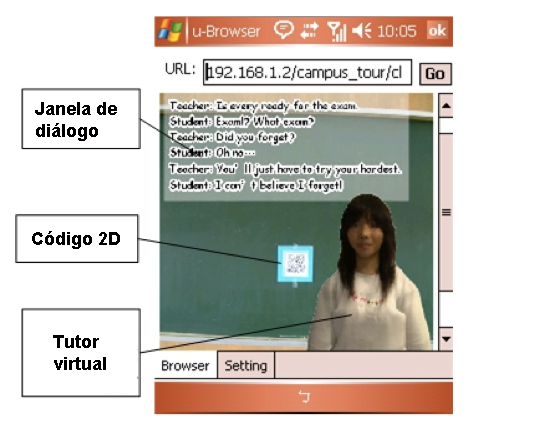
\includegraphics[scale=.7]{figuras/cap2/hello.png}
		\caption{\textit{Exemplo do tutor virtual utilizado no HELLO. Adaptado de~\cite{tsung}.}}
		\label{fig:hello} 
	\end{figure}
	\subsection{SmARt World}
\label{sec:smart}

	\textit{SmARt World} é um \textit{framework} voltado para a computação ubíqua, ao qual utiliza a 
	Realidade Aumentada com o objetivo de criar novos conteúdos virtual e interação com o ambiente
	inteligente~\cite{yew}. Outro objetivo desse \textit{framework} está no auxílio da construção de
	aplicações voltada para a Realidade Aumentada baseada em dispositivos móveis, tornando esse
	desenvolvimento simplificado. O \textit{framework} é capaz de criar e apresentar objetos virtuais
	ao usuário, provendo uma interação por meio destes. Sua arquitetura é dividida em: 
	
	%Sua arquitetura é ilustrada conforme a
	%figura~\ref{fig:arquitetura_smart}.
	
	%\begin{figure}[htb]
	%	\centering 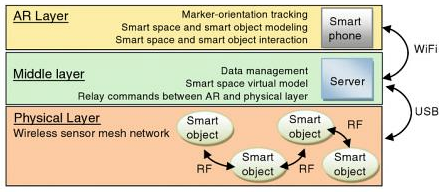
\includegraphics[scale=0.8]{figuras/cap2/arquitetura_smart.png}
	%	\caption{\textit{Arquitetura do framework SmARt World \cite{yew}.}}
	%	\label{fig:arquitetura_smart}
	%\end{figure}
	
	\begin{enumerate}
	  \item \textbf{Camada Física}
	  	
	  	Nessa camada os objetos inteligentes são interligados através de transmissores de rádio
	  	frequência, onde estes são ligados um nó central que faz acesso a Camada Intermediária. Esse nó
	  	central também fica responsável por reconhecer os demais nós ativos na rede, controlar as
	  	informações que são repassadas pelos nós e posteriormente enviar os dados a Camada Intermediária
	  	para que as informações correspondentes aos nós sejam atualizadas.
	  	
	  	Cada transmissor possui seu código identificador para se comunicar com a rede, essa comunicação
	  	é feita através de sensores ou por comunicações interligadas fisicamente. O objetivo da
	  	utilização desses transmissores acoplados aos dispositivos possibilita o controle dos
	  	mesmos, acrescentando uma inteligência a rede. Desta forma, de acordo com a informação captada
	  	pelos transmissores, é possível enviar sinais específicos para os dispositivos. Esse controle
	  	será feito através da interface provida pelo~\textit{smartphone}, na Camada AR.
	  
	  \item \textbf{Camada Intermediária}
	  
	  	Essa camada possui a responsabilidade de armazenar e gerenciar todas as informações a respeito
	  	do ambiente inteligente e dos usuários e objetos pertencentes a ele. A comunicação entre a
	  	aplicação e os demais componentes da rede é feita através de uma interface web que
	  	disponibiliza acesso a aplicação e ao banco de dados contido em servidor. O banco de dados
	  	armazena informação a respeito do objeto, tais como: posicionamento, modelagem 3D, textos
	  	apresentados ao usuário, formato e contexto. 
	  
	  \item \textbf{Camada AR}
	
		Essa camada utiliza uma aplicação voltada para a Realidade Aumentada que é capaz de
		rastrear e reconhecer os marcadores. Através disso possibilita uma interação entre os
		objetos virtuais e reais. Essa camada foi projetada para ser utilizada em dispositivos móveis.
		Por essa razão, o protótipo para essa camada foi desenvolvido para a plataforma Android.
		
	\end{enumerate}
	
	\subsubsection{Marcadores e a Realidade Aumentada}
	
	O rastreamento e reconhecimento dos marcadores é feito a partir de dois métodos combinados. O
	primeiro é o reconhecimento dos objetos através do uso de marcadores. Após o reconhecimento, o
	segundo método é iniciado. Neste, sensores são utilizados para obter a orientação e posicionamento
	do objeto. Esse posicionamento é gravado na Camada Intermediária através das coordenadas \{x,y,z\}. O
	\textit{framework} possui a funcionalidade de seleção de objetos virtuais através da tela do
	\textit{smartphone}, possibilitando redefinir o novo posicionamento do objeto virtual selecionado
	no ambiente inteligente.
	
	
	
	
	
